%#! latexmk -lualatex -synctex=1
% !TeX program = lualatex
\documentclass[lualatex,fleqn]{uitex}

% 数式関連
\usepackage{mathtools,amssymb,unicode-math}

% フォント
\usepackage[match,deluxe,expert]{luatexja-preset}
\setmainfont{TeX Gyre Termes}
\setmathfont{TeX Gyre Termes Math}
\setsansfont{TeX Gyre Heros}
\setmonofont[FakeStretch=.8748]{Source Code Pro}

% 画像の取り込み，図表の配置
\usepackage{graphicx,subcaption}
\usepackage{array}

% URL
\usepackage{url}
\DeclareUrlCommand\url{%
  \def\UrlLeft{<}\def\UrlRight{>}\urlstyle{rm}}

% ロゴ関連
\usepackage{hvlogos,metalogox}

% 色付きボックス
\usepackage[most]{tcolorbox}

% 国際単位系
\usepackage{siunitx}

% 最後のページの行数を揃える
\usepackage[checkfloat]{flushend}

% 便利マクロ集
\usepackage{mknmacro}

% 文字のアキを調整する
\ltjsetparameter{alxspmode={`*,allow}}
\ltjsetparameter{alxspmode={`\\,allow}}
\ltjsetparameter{alxspmode={`\{,allow}}
\ltjsetparameter{alxspmode={`\},allow}}

% サンプル文書用マクロ
\DeclareRobustCommand\UiTeXcls{\texttt{uitex.cls}}

\title{%
  職業能力開発研究発表講演会に提出する発表論文を作成するための\\
  {\LuaLaTeX}用私家版クラスファイル{\UiTeXcls}の使いかた}
\author{%
  ○上羽 未栞，橘 紗鳥，緋本 奈緒（み研究所）}

\pagestyle{forum}% 発表論文の体裁
\ForumNumber{36}% 第何回
\ForumDate{2026/11/27\,〜\,28}% 開催日

\setlength{\leftmargini}{1\zw}

\begin{document}

\maketitle

\section{はじめに}

\begin{tcolorbox}[
    enhanced,
    left skip=.5\zw,
    boxsep=0pt,
    frame engine=empty, boxrule=0pt,
    left=\dimexpr1.5\zw+.25mm\relax, right=0pt,
    sharp corners,
    borderline west={.5mm}{0pt}{black!75!white},
    colback=white]
  だってやっぱ最初のね\\
  印象大事がイマなので\par
  \hfill--- AMAMOGU『バチモリーナ』（2025）
\end{tcolorbox}

本稿では，
某大学校において例年開催される「PTUフォーラム」の
「職業能力開発研究発表講演会」に提出する発表論文を
{\LuaLaTeX}で作成するための私家版クラスファイル
{\UiTeXcls}の使いかたについて説明します．

{\LaTeX}のインストール方法や
{\LaTeX}を使った文書の作成方法については，
\文献{TeXWiki,美文書}などを参照してください．
発表論文を作成する上での注意事項については，
某大学校のウェブサイト上の
「基盤整備センター」の「PTUフォーラム」のページ\cite{PTUForum}で
例年配布されている「発表申し込み・論文の提出・発表について」や
「論文テンプレート」に記載されている内容を参照してください．

発表論文を作成するにあたって，
「発表申し込み・論文の提出・発表について」には，
「テンプレートをダウンロードしてご使用ください」とあります．
このクラスファイルを使って得られた組版の結果は，
上で述べられているテンプレートを用いた組版の結果と異なるかもしれません%
\footnote{実際，誌面の見栄えを良くするために，
  指定されているものと異なる書式を設定している箇所があります．}．
発表論文の作成者は，
これを理解し，
自らの判断のもとにこのクラスファイルを使ってください．

なお，このクラスファイルに関する詳細なライセンスについては，
クラスファイルに同梱されるファイル\texttt{LICENSE}を参照してください．

以降，
\ref{sec:クラスファイルの説明}で
このクラスファイルや関連する各種のパッケージについて，
\ref{sec:発表論文を作成する上での注意}で
発表論文を作成する上での注意点について説明します．
\ref{sec:追加のマクロ}では，便利なマクロ集について軽く触れます．
最後に，
\ref{sec:おわりに}でこのクラスファイルの今後の展望や
バグの対応について述べます．

\section{クラスファイルの説明}
\label{sec:クラスファイルの説明}

クラスファイル{\UiTeXcls}は，
「PTUフォーラム」の
「職業能力開発研究発表講演会」の発表論文のための体裁を提供します．
このクラスファイルの最新版をGitHub~\cite{uitex}から取得できます．
なお，このクラスファイルは，
阿部紀行氏によって開発された\verb|jlreq|~\cite{jlreq}をラップしたものです．

\subsection{テンプレートと記述方法}

\begin{figure}[tb]
  \begin{tcblisting}{listing only, top=1ex, bottom=1ex, left=.5em, right=.5em}
\documentclass[lualatex,fleqn]{uitex}
\usepackage{mathtools,amssymb,unicode-math}
\usepackage[match,deluxe,expert]{luatexja-preset}
\setmainfont{TeX Gyre Termes}
\setmathfont{TeX Gyre Termes Math}
\setsansfont{TeX Gyre Heros}
\setmonofont[FakeStretch=.8748]{Source Code Pro}
\usepackage{mknmacro}
\title{論文タイトル\\改行もできます}
\author{%
  ○能開 花子，教育 一郎（某大学校），%
  研究 二郎（某未来技研），\\% 改行できます
  発明 三郎（某製作所）}
\pagestyle{forum}% 発表論文の体裁
\ForumNumber{36}% 第何回
\ForumDate{2026/11/27\,〜\,28}% 開催日
\begin{document}
\maketitle
\section{はじめに}
ほげほげ……
\begin{thebibliography}{9}
  \bibitem{hoge}
    ふがふが……
\end{thebibliography}
\end{document}
  \end{tcblisting}
  \vspace{-.25\baselineskip}
  \caption{記述例}
  \label{fig:example}
\end{figure}

必要最低限の記述例を\図{fig:example}に示します．
このクラスファイルに同梱されるファイル
\texttt{template.tex}や\texttt{readme.tex}を併せて参照してください．

それぞれの記述について，順に説明します．

\begin{itemize}
  \item
    ドキュメントクラスに\verb|uitex|を指定します．
    併せて，クラスオプションを指定します．
    {\LuaLaTeX}で組版することを明示するために\verb|lualatex|を，
    数式を左側に寄せて表示するために\verb|fleqn|を指定します．
    この他にも，
    \verb|jlreq|クラスが受け付けるようなオプションを指定できます．
  \item
    数式に関連するいくつかのパッケージを指定します．
    \verb|mathtools|パッケージ及び\verb|amssymb|パッケージは，
    数式に関連する様々な機能や記号を提供します．
    \verb|unicode-math|パッケージは，数式用のフォントを設定します．
    本稿の\ref{sec:高度な数式}を併せて参照してください．
  \item
    フォントに関連するパッケージを指定し，設定を行います．
    \verb|luatexja-preset|パッケージは，
    和文フォントに関連する設定を行います．
    詳細については，
    {\LuaTeX}-jaパッケージのドキュメントを参照してください
    （\verb|texdoc luatexja|）．
    続いて，欧文フォントの設定を行います．
    {\TeX} Gyreフォント集を使います．
    メインフォント及び数式フォントにTimes相当のTermesを，
    サンセリフフォントにHelvetica相当のHerosを指定します．
    等幅フォントには，横幅を潰したSource Code Proを指定します．
  \item
    図表などの参照や数式中の括弧などに関連する便利なマクロを使うには，
    \verb|mknmacro|パッケージを指定します．
    本稿の\ref{sec:追加のマクロ}を併せて参照してください．
  \item
    \verb|\title|で発表論文の題目を指定します．
    \verb|\\|を使って改行できます．
  \item
    \verb|\author|で発表論文の著者を指定します．
    各著者を全角カンマ（，）で区切り，
    所属を全角丸括弧「（」「）」で囲みます．
    やはり\verb|\\|で改行できます．
  \item
    \verb|\pagestyle|で発表論文の体裁を指定します．
    \verb|forum|を指定することで，
    職業能力開発研究発表講演会用の体裁になります．
  \item
    \verb|\ForumNumber|及び\verb|\ForumDate|で
    PTUフォーラムの開催される回，及び日付をそれぞれ指定します．
    \verb|\ForumDate|に指定する日付の「〜」の両側に
    狭いアキ（\verb|\,|）を置いておくと，
    より見栄えよく仕上がります．
    ヘッダに表示される「PTUフォーラムYYYY」の「YYYY」の部分は，
    \verb|\ForumDate|で指定された文字列のうち，
    半角スラッシュ（\verb|/|）に初めて遭遇するまでの部分を
    切り出して自動的に設定されます．
  \item
    \verb|\begin{document}|と\verb|\end{document}|との間に本文を記述します．
    なお，\verb|\maketitle|で発表論文の題目と著者一覧とが出力されます．
\end{itemize}

\subsection{コンパイル方法}

{\LuaLaTeX}を使ってコンパイルする必要があります．
最も単純には，次のコマンドを実行します．
ただし，\texttt{\itshape template.tex}の部分は，
適当に置き換えます．
この方法では，
正しい組版結果を得るために，
コマンドを複数回実行する必要があります．
\begin{tcblisting}{listing only, top=1ex, bottom=1ex, left=.5em, right=.5em}
$ lualatex template.tex
\end{tcblisting}

あるいは，latemkxを使って
必要なコマンドを必要な回数だけ自動的に実行します．
やはり，\texttt{\itshape template.tex}の部分は，
適当に置き換えます．
\begin{tcblisting}{listing only, top=1ex, bottom=1ex, left=.5em, right=.5em}
$ latexmk -lualatex template.tex
\end{tcblisting}

さらに，このクラスファイルに同梱されるファイル
\texttt{template.tex}や\texttt{readme.tex}は，
ファイルの冒頭部分に{\TeX}-style shebangをもっていますから，
\texttt{runtexshabeng}コマンドを実行することで，
latexmkを実行できます．
\begin{tcblisting}{listing only, top=1ex, bottom=1ex, left=.5em, right=.5em}
$ runtexshebang template.tex
\end{tcblisting}

なお，このクラスファイルそれ自体は，
{(u)p\LaTeX}においても使えます．
しかし，{(u)p\LaTeX}は，古い{\LaTeX}処理系です．
よほどの理由がないかぎり，{\LuaLaTeX}を使ってください．
同梱されるファイル\texttt{template.tex}や\texttt{readme.tex}は，
{\LuaLaTeX}専用です．

\subsection{{\TeX}worksを使う際の注意}
\label{sec:TeXworksを使う際の注意}

クラスファイルに同梱されるファイル
\texttt{template.tex}や\texttt{readme.tex}は，
ファイルの冒頭部分に{\TeX}worksのためのmagic commentをもっています．
したがって，
これらのファイルを{\TeX}worksで開くと，
適切な{\LaTeX}エンジン（{\LuaLaTeX}）が選択されるはずです．
これ以外の{\LaTeX}エンジンが選択される場合は，
\図{fig:texworks}のように手動で{\LaTeX}エンジンを選択しなおす必要があります．
また，正しい組版結果を得るためには，
複数回のコンパイルが必要になる場合があります．

\begin{figure}[b]
  \centering
  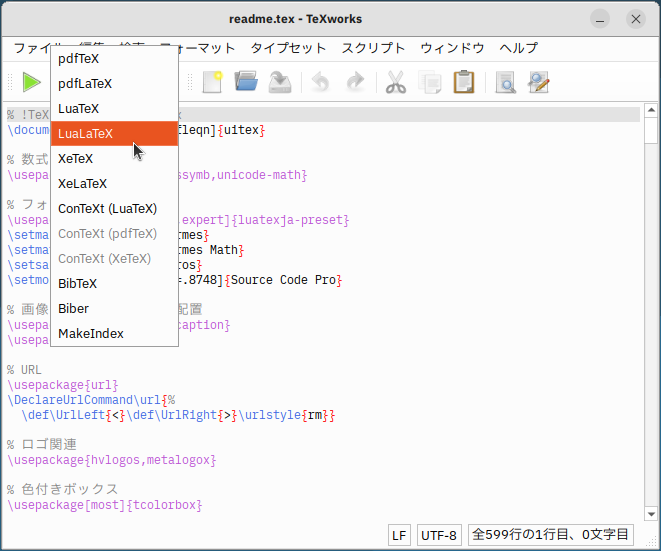
\includegraphics[width=.9\linewidth]{./figures/texworks.png}
  \caption{{\LaTeX}エンジンとして{\LuaLaTeX}を選択する}
  \label{fig:texworks}
\end{figure}

\subsection{見出し}

見出しが連続する場合の処理を実装しています．
つまり，\verb|\section|の直後に\verb|\subsection|が続くなどする場合，
「論文テンプレート」の3.と3.1.との間や3.4.と3.4.1.との間のように，
適切なアキとなるように設定されています．

\subsection{数式}

ディスプレイ数式は，
\式{eq:example}のように表示されます．
数式を丸括弧付きで参照するために，
\verb|\eqref|を使うと便利です．
数式を独立した段落として表示することを望まない場合，
数式の直前の文と数式との間に空行を置かないでください．
さもなくば，不自然なアキが発生して不恰好に見えます．
\begin{equation}
  \zeta\pq{s}
  \coloneq \sum_{n=1}^{\infty} \frac{1}{n^s}
  = \frac{1}{1^s} + \frac{1}{2^s} + \frac{1}{3^s} + \frac{1}{4^s} + \cdots
  \label{eq:example}
\end{equation}

\subsubsection{高度な数式}
\label{sec:高度な数式}

\verb|mathtools|パッケージを用いることで，
より高度な数式を記述できます．
\verb|mathtools|パッケージは，
\verb|amsmath|パッケージを内部で読み込みます．

\verb|unicode-math|を用いていますから，
数式中で$\symbfit{v}$や$\symbfit{M}$，
$\symbfit{\lambda}$などの太字を表示するには，
\verb|\symbfit|を用います．

\subsection{図表}

\begin{figure*}[tb]
  \begin{subfigure}{.5\linewidth}
    \centering
    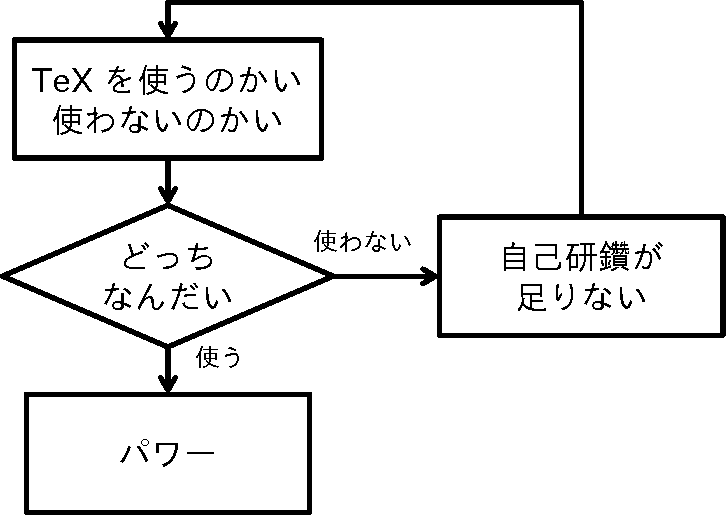
\includegraphics[width=.8\linewidth]{./figures/power.pdf}
    \caption{ベクタ形式（PDF）}
    \label{fig:vector}
  \end{subfigure}
  \begin{subfigure}{.5\linewidth}
    \centering
    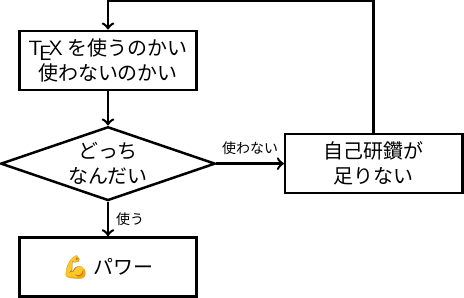
\includegraphics[width=.8\linewidth]{./figures/power.png}
    \caption{ラスタ形式（PNG）}
    \label{fig:raster}
  \end{subfigure}
  \caption{図の比較}
  \label{fig:compare}
\end{figure*}

図や表を配置するために，
\verb|figure|環境や\verb|table|環境を用います．
二段抜きの場合は，
\verb|figure*|環境や\verb|table*|環境を用います．
\verb|[t]|や\verb|[tb]|のように，
出力位置を指定するためのオプションを必ず指定してください．
\図{fig:compare}のように図表に副番号を添えたい場合は，
\verb|subcaption|パッケージを用いると便利です．

\subsubsection{画像の取り込み}

\verb|graphicx|パッケージを用いることで，
画像を取り込めます．
ブロック図やグラフなど，
線による描画が主である画像を取り込む場合，
PDFやEPSなどのベクタ形式の使用を検討してください．
ベクタ形式の図は，
拡大してもボヤけずに表示できます．
\図{fig:vector}と\図{fig:raster}とを比較してください．
図を取り込む際，
\verb|width=\linewidth|のオプションを指定すると，
行の幅一杯に画像を表示できます．
\文献{美文書}の第7章を併せて参照してください．

\subsubsection{PDFの切り抜き}

\verb|pdfcrop|コマンドを用いることで，
PDFファイルの余白を削除できます．
このコマンドは，
{\TeX} Liveに含まれています．
例えば，次のコマンドを実行すると，
\texttt{file.pdf}の余白を削除したファイル
\texttt{file-crop.pdf}を生成できます．

\begin{tcblisting}{listing only, top=1ex, bottom=1ex, left=.5em, right=.5em}
$ pdfcrop file.pdf
\end{tcblisting}

\subsubsection{{\TikZ}による描画}

{\TikZ}を用いるには，
\verb|tikz|パッケージを指定します．
{\TikZ}を用いることで，
{\LaTeX}文書中に図を直接記述できます．
フローチャートのようなブロック図を描画する際には，
専用のグラフィックソフトを利用するよりも手っ取り早く図を用意できます．
\図{fig:vector}の元画像は，
{\TikZ}によって記述されています．
このクラスファイルに同梱される\texttt{figure/power.tex}を参照してください．
{\TikZ}の詳細については，
\文献{美文書}の付録Dや\文献{tikz}などを参照してください．

\subsubsection{表の記述}

表の内容は，
少し小さい文字（\verb|\small|）で組まれます．
\図{fig:table}のように記述することで，
\表{tab:chugoku}を得られます．
表の一番上及び一番下の罫線を太くするため，
\verb|\Hline|を用いてください．
\verb|array|パッケージを用いることで，
表の描画が若干修正されます．
また，\verb|tabularray|パッケージを用いることで，
表をより柔軟に記述できます．
詳細については，
\文献{美文書}の第8章を参照してください．

\begin{figure}[tb]
  \begin{tcblisting}{listing only, top=1ex, bottom=1ex, left=.5em, right=.5em}
\begin{table}[tb]
  \centering
  \caption{中国地方の都道府県}
  \label{tab:chugoku}
  \begin{tabular}{ccr}
    \Hline
    県名 & 県庁所在地 & 人口\Cite{人口} \\
    \hline
    鳥取県 & 鳥取市 &   531千 \\
    島根県 & 松江市 &   642千 \\
    岡山県 & 岡山市 & 1,831千 \\
    広島県 & 広島市 & 2,714千 \\
    山口県 & 山口市 & 1,281千 \\
    \Hline
  \end{tabular}
\end{table}
  \end{tcblisting}
  \vspace{-.25\baselineskip}
  \caption{表の記述例}
  \label{fig:table}
\end{figure}

\begin{table}[tb]
  \centering
  \caption{中国地方の都道府県}
  \label{tab:chugoku}
  \begin{tabular}{ccr}
    \Hline
    県名 & 県庁所在地 & 人口\Cite{人口} \\
    \hline
    鳥取県 & 鳥取市 &   531千 \\
    島根県 & 松江市 &   642千 \\
    岡山県 & 岡山市 & 1,831千 \\
    広島県 & 広島市 & 2,714千 \\
    山口県 & 山口市 & 1,281千 \\
    \Hline
  \end{tabular}
\end{table}

\subsubsection{色付きの枠}

\verb|tcolorbox|パッケージを用いることで，
色付きの枠を表示できます．
本稿の冒頭の引用句の飾り枠は，
\verb|tcolorbox|環境によって実現されています．
また，本稿においてソースコードを示すために使っている枠は，
当該パッケージの\verb|tcblisting|環境によって実現されています．
日本の{\LaTeX}において古くから使われている\verb|ascmac|パッケージに比べて，
柔軟にカスタマイズできるなどの特徴があります．
\文献{美文書}の第7章に簡単な説明があります．
詳細については，
ドキュメントを参照してください（\verb|texdoc tcolorbox|）．

\subsection{参考文献}

参考文献リストの記述が特殊であるため，
{\BibTeX}の使用を推奨できません．
手動で\verb|thebibliography|環境に文献リストを入力してください．
文献を引用するための\verb|\cite|は，
通常の（つまり，上付きでない）引用です．
「\verb|文献\cite{uitex}|」は，「文献\cite{uitex}」のように表示されます．
上付きの引用は，
\verb|\Cite|を用いることで簡単に実現できます．
「\verb|文献\Cite{uitex}|」は，この文末のように表示されます\Cite{uitex}．

\subsection{注釈}

本稿の冒頭で使っていたように，
脚注\footnote{脚注は，このように表示されます．}を使えます．
使い所に迷いますが，
割注\warichu{このような見た目で挿入される注}も使えます．
詳細については，\文献{jlreq}を参照してください．

\section{発表論文を作成する上での注意}
\label{sec:発表論文を作成する上での注意}

和文中の句読点や括弧類は，
全角のもの（，）（．）「（」「）」を使ってください．
半角のもの（,）（.）「(」「)」を使うと，
文字の幅や高さが合わなくなり，
見苦しくなります．
特に，参考文献リストにおける和文の項目については，
全角の句読点や括弧類を使ってください．
欧文中の句読点や括弧類は，
半角のものを使ってください．
半角のクオート（`）（'）（``）（''）を表示するには，
それぞれ（\verb|`|）（\verb|'|）（\verb|``|）（\verb|''|）
のように記述してください．

ハイフンとダーシとをきちんと使い分けてください．
ハイフン（\verb|-|）は，
主に二つの単語を接続する用途で使います（well-knownなど）．
二分ダーシ（\verb|--|）は，
主に範囲を表す用途で使います（pp.29--57など）．

単位の直前（1個の個の直前）や
図表などの参照の途中（表1の表の直後）で改行されると見苦しいですから，
そのような箇所には\verb|\nolinebreak|を挿入したり，
改行できる箇所に\verb|\linebreak|を挿入したりして回避してください．
\ref{sec:参照}を併せて参照してください．
また，改行（\verb|\\|）を濫用しないでください．

\subsection{美しい文書を作成するための便利なパッケージ}

国際単位系を用いる場合には，
\verb|siunitx|パッケージが便利です．
これは，単位の直前のアキを適切に制御してくれます．
例えば，「\verb|\qty{1}{\milli\metre}|」は，
「\qty{1}{\milli\metre}」のように表示されます．
詳細については，
ドキュメントを参照してください（\verb|texdoc siunitx|）．

URLを表示する場合には，
\verb|url|パッケージが便利です．
本稿では，
URLの先頭と末尾とを判りやすくする山括弧を表示するため，
以下の設定を添えています．
例えば，「\verb|\url{https://example.com/}|」は，
「\url{https://example.com/}」のように表示されます．
詳細については，
ドキュメントを参照してください（\verb|texdoc url|）．
\begin{tcblisting}{listing only, top=1ex, bottom=1ex, left=.5em, right=.5em}
\DeclareUrlCommand\url{%
  \def\UrlLeft{<}\def\UrlRight{>}\urlstyle{rm}}
\end{tcblisting}

\文献{w3c}によれば，
「改丁や改ページなどの直前のページにおいて，
段組の行がページの途中で終わる場合は，（中略）
横組の場合は，各段の行数を平均にする．」とあります．
\文献{jlreq}では，
これを実現するために
\verb|nidanfloat|パッケージを用いた例が示されていますが，
上手く動作しません．
\verb|flushend|パッケージを用いることで，
これを実現します．
オプションに\verb|checkfloat|を添えて，
図表のフロートに関する処理を行うよう指示します．
また，\verb|\flushcolsend|を\verb|\end{document}|の直前に置いておきます．
仕上がりは，本稿の最後のページのようになります．

\section{追加のマクロ}
\label{sec:追加のマクロ}

クラスファイル{\UiTeXcls}に加え，
スタイルファイル\texttt{mknmacro.sty}を同梱しています．
このファイルには，
いくつかの便利なマクロを収録しています．

\subsection{数式中の括弧}

数式中で使う括弧類のマクロを定義しています．
これらのマクロのために，
\verb|mathtools|パッケージを内部で用いています．
例えば，「\verb|$a+\brq{b+\bq{c+\pq{d+e}}}$|」は，
「$a+\brq{b+\bq{c+\pq{d+e}}}$」のように表示されます．
これらのマクロは，
星付きの名前（\verb|pq*|など）で使われた際に，
括弧の中身に応じて自動的に括弧のサイズを調整します．
例えば，\verb|y = \pq*{\frac{x+1}{x}}^{x}|は，
\式{eq:pq}のように表示されます．
\begin{equation}
  y = \pq*{\frac{x+1}{x}}^{x}
  \label{eq:pq}
\end{equation}

「\verb|\left(|」や「\verb|\right)|」によって同様のことを実現できますが，
これはタイプする文字が多いだけでなく，
括弧の周りに不自然なアキを発生させてしまいます．
\texttt{mknmacro}パッケージで定義されるマクロでは，
そのようなアキは発生しません．

括弧のほかに，
絶対値（\verb|\abs|）や床関数（\verb|\floor|），
天井関数（\verb|\ceil|）をも用意しています（\式{eq:ceil}）．
\begin{equation}
  \ceil*{\frac{a\vphantom{1}}{b}}\
  = \floor*{\frac{a+b-1}{b}}
  = \floor*{\frac{a-1}{b}}+1
  \label{eq:ceil}
\end{equation}

\subsection{参照}
\label{sec:参照}

参照を表示するためのマクロ
（\verb|\図|，\verb|\表|，\verb|\式|，
及び\linebreak\verb|\文献|）を定義しています．
例えば，「\verb|\図{fig:table}|」は，
「\図{fig:table}」のように表示されます．
波括弧の中には，
\verb|\ref|や\verb|\cite|と同様の引数を指定します．
「図3」の「図」と「3」との間で改行されてしまうと見苦しいですから，
これらを抑制するように定義しています．

\section{おわりに}
\label{sec:おわりに}

本稿では，
某大学校において例年開催される「PTUフォーラム」の
「職業能力開発研究発表講演会」に提出する発表論文を
{\LuaLaTeX}で作成するためのクラスファイル
{\UiTeXcls}の使いかたについて説明しました．

某大学校においては，
この書式に酷似した原稿を用意する場面が少なくないと思われます．
今後，そのような場面においてもこのクラスファイルを利用できるよう，
修正を重ねていく予定です．
また，このクラスファイルを利用していて意図しない組版結果となる場合や
クラスファイルに問題があると思われる場合には，
\文献{uitex}からissueを作成して報告してください．

おわりです．

\begin{thebibliography}{9}
  \bibitem{TeXWiki}
    ``{\TeX} Wiki'',
    \url{https://texwiki.texjp.org/},
    accessed in 2026-09.
  \bibitem{美文書}
    奥村晴彦，黒木裕介：
    「［改訂第9版］{\LaTeX}美文書作成入門」，
    株式会社技術評論社，
    東京
    （2023）．
  \bibitem{PTUForum}
    職業能力開発総合大学校：
    「PTUフォーラム」，
    基盤整備センター，
    \url{https://www.uitec.jeed.go.jp/kiban/research/}，
    2026-09参照．
  \bibitem{uitex}
    KusaReMKN:
    ``KusaReMKN/uitex'',
    GitHub,
    \url{https://github.com/KusaReMKN/uitex},
    accessed in 2026-09.
  \bibitem{jlreq}
    N.~Abe:
    ``abenori/jlreq'',
    GitHub,
    \url{https://github.com/abenori/jlreq},
    accessed in 2026-09.
  \bibitem{tikz}
    Stefan Kottwitz，
    黒川利明 訳：
    「{\TikZ}による{\LaTeX}グラフィックス」，
    株式会社朝倉書店，
    東京
    （2024）．
  \bibitem{人口}
    総務省統計局：
    「人口推計（2024年（令和6年）10月1日現在）」，
    \url{https://www.stat.go.jp/data/jinsui/2024np/index.html}，
    （2025）．
  \bibitem{w3c}
    千葉弘幸ら：
    「日本語組版処理の要件（日本語版）」，
    \url{https://www.w3.org/TR/jlreq/},
    （2020）．
\end{thebibliography}

\flushcolsend
\end{document}
% mkn: forceComma forcePeriod :
% ex: se et ts=2 :
